\section{Introduction}
As the world population keeps on growing, so does the need for energy. The increasing demand of energy requires more sustainable and efficient energy production methods as the amount of air pollution must decrease which is stated by the Paris climate accord. So the challenge at this moment is not only generating more power, it is also about generating energy with less pollution or even better, without any pollution. The use of power technologies that integrate carbon capture such as the Allam Cycle and the Argon Power Cycle (APC) are gaining interest. In the case of the latter, polymeric membrane separation is a promising technology for cost-effective integration of carbon capture onto large size internal combustion engines used today to compensate intermittent renewable sources. \\
The APC is an innovative technology which either improves thermodynamic efficiency and reduces emission. This is achieved by replacing air with argon as working fluid. Other noble gases such as helium could be used as well, but argon is preferred due to its abundance, non-toxicity and relatively low cost compared to other gases. The increase in thermal efficiency mostly relies on the high specific heat ratio of mono-atomic gases. The influence of the specific heat ratio on the thermal efficiency is clearly apparent in the \textit{Otto-cycle} where the efficiency is described with:
\vspace{-0.3cm}
\begin{align}
	&&\eta = 1 - \frac{1}{r^{\kappa - 1}}
\end{align}
Although hydrogen is the perfect fuel for the APC because it does not produce carbon dioxide, it suffers from knocking. Due to high heat capacity ratio, the auto-ignition temperature is reached at relatively low compression ratio \textit{r} and this can lead to knocking. Methane offers a good solution to this problem. \\ 

The gasses of $CO_2$, $H_2O$ and \textit{Ar} should be separated from the exhaust stream to achieve a closed loop combustion of methane. The first separation stage is done using a condensation unit through which water is removed from the system. The innovation in this work consists of the use of membrane separation. The remaining $CO_2$ and $Ar$ are separated using a set of membranes and compressors. This results in a high purity stream of $CO_2$ (95$\%$), which may be injected in $CO_2$ pipelines for further use in Enhanced Oil Recovery (EOR) or in chemical processes.  \cite{Chourou2017}

\begin{figure}[H]
	\centering
	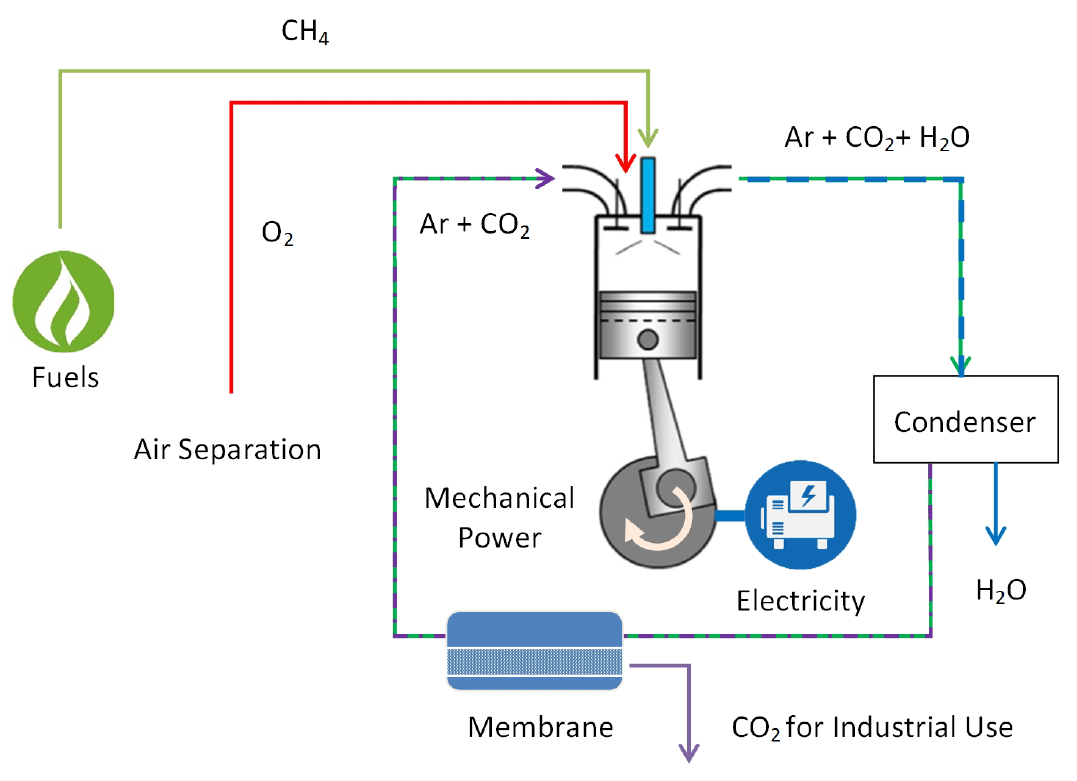
\includegraphics[width= 1\textwidth]{Images/fig8.png}
	\captionof{figure}{Basic process diagram of APC in a methane energy storage scheme \cite{Chourou2017}}
	\label{fig:fig8}
\end{figure}

To investigate the process, a one dimensional model which accounts for mass and species conservation is developed and solved using Finite Volume Method (FVM) in MATLAB$^\circledR$. The target is to develop a simplified code for transient APC systems. \\

A non-polluting powerplant would provide several benefits, but the most important one is that there is less need for flexibility as it could operate without time constraints from the government. 